\section{Other Case Studies}

\subsection{Nile Water Conflict}

\paragraph{Background}

\subparagraph{Geographical Background}

Nile: one of the longest rivers in the world

\begin{itemize}
    \item Passes through 11 countries, over 250 million people live in the Nile basin
    \item 95\% of Egypt population rely on Nile's water
    \item Two main tributaries:
        \begin{itemize}
            \item White Nile - long stream, originating from Lake Viktoria
            \item Blue Nile - provides 2/3 of the Nile's water, originates
                in Ethiopia.
        \end{itemize}
\end{itemize}

\subparagraph{Historic Background}

\begin{itemize}
    \item Allocation of Nile's estimated 84 km$^3$ water per year, measured
        at Aswan High Dam, Eqypt.
    \item Egypt claims veto rights to upstream projects impacting the Nile's flow
    \item Treaty not recognized by Ethiopia.
\end{itemize}

\subparagraph{Matter of Dispute: Grand Ethiopian Renaissance Dam}

\begin{itemize}
    \item Since 2011, Ethiopia is constructing Africa's largest hydropower
        plant and the world's 7th largest artificial lake. Main dam 1800 m
        long, 145 m high, side dam 5000 m long, 50 m high.
    \item Potential to increase Ethiopia's generation capacity by 6450 MW
        (currently 4200 GW)
        \begin{itemize}
            \item Currently over 60\% of Ethiopians not connected to the grid
            \item Potential to become Africa's largest power exporter
        \end{itemize}
    \item 79 km$^3$ water in reservoir: Almost the size of lake Geneva and
        more than annual flow of Blue Nile.
    \item Blue Nile main source of the Nile's water $\rightarrow$ depending
        on filling regime, Nile flow can be impacted severely.
\end{itemize}

\paragraph{Negotiation}

\subparagraph{Ethiopia}
\begin{itemize}
    \item No international financing: Symbol of national pride
    \item Meet electricity demand and export power
    \item Dam at core of industrial plans and economic growth
    \item Filling over 7 years: Reduce Nile flow by up to 25\%
\end{itemize}

\subparagraph{Egypt}
\begin{itemize}
    \item Claiming historic right to Nile waters and veto right to any upstream
        project
    \item Fears drop of own hydropower generation and damage to agriculture
    \item The dam gives Ethiopia leverage
    \item Filling over 12-21 years
\end{itemize}

\subparagraph{Sudan}
\begin{itemize}
    \item Dam will help control Blue Nile flow $\rightarrow$ manage annual floods
    \item Reduce electricity deficit by importing power
\end{itemize}

\pagebreak

\hrule

\subsubsection{Excursion: General Safeguard Clause}

What happens in special situations, when one party can not stick to treaty
due to serious difficulties? Tried and tested tool: Safeguard clause.
Example: European Economic Area (EEA): Safeguard measures, Art. 112

\begin{enumerate}[]
    \item \underline{Benefits}: Generally applicable, Unilaterally invokable
    \item \underline{Disadvantages}: Not concrete, abstract, Dispute: When are difficulties "serious"?
\end{enumerate}
In the Nile case, it is possible to define "serious difficulties" more concretely.

\paragraph{Specific Safeguard Clause}

Agreements describe general principles and mechanisms. Consider a normal
distribution. When normal situation is clearly defined, mechanisms can be
agreed on that apply in extreme situations.
One example is the Land transport Agreement EU-CH: Article 46.

\begin{enumerate}[]
    \item \underline{Benefits}: No room for interpretation, clear,
        Even if never invoked, provide security against potential negative
        events
    \item \underline{Disadvantages}: Not general, requires precise definitions,
        Consists of trigger conditions and measures.
\end{enumerate}

\hrule

\paragraph{Possible Solutions}

\begin{itemize}
    \item What should be the Blue Nile's minimum annual flow?
    \item Definition of safeguard clauses:
        \item What is drought, extended drought, severe drought?
        \item Guaranteed minimum filling level of Egypt's own Aswan high Dam?
        \item Parameter causing issue: Too little water
        \item Of the two cases distinguished, here it is possible to be more specific.
\end{itemize}

\subparagraph{Possible Safeguard Clause}

If\dots
\begin{itemize}
    \item GERD lake lavel at least \dots m $\rightarrow$ Conditions
\end{itemize}
And\dots
\begin{itemize}
    \item GERD water releases below certain norm
    \item Precipitation in current season below norm
    \item Mean temperature consistently above norm
    \item $\rightarrow$ Triggers (No room for interpretation!)
\end{itemize}
Then\dots
\begin{itemize}
    \item GERD release must be at least \dots m$^3$/day
    \item Additional release proportional ot difference between current
        filling level and defined minimum filling level.
    \item $\rightarrow$ Appropriate measures
\end{itemize}

\paragraph{Conclusion: Take-aways}

\begin{itemize}
    \item Classic negotiation scenario
    \item Conflicts over water will become increasingly relevant
    \item Engineering approach does not solve the problem, but makes it more objective
    \item "Reduce problem to its most formal structure"
\end{itemize}


\subsection{Brexit}

\paragraph{a) Background}

\subparagraph{Milestones}

\begin{itemize}
    \item 19 Feb 2016: PM Cameron and Com Pres Juncker redraw the terms
        of the UK's membership
        \begin{itemize}
            \item Restricted access to in-work benefits for EU migrants
            \item Child benefit payments indexed to the cost of living
                for children living outside the UK for all new arrivals
            \item References to "ever-closer union" do not apply to the UK
        \end{itemize}
    \item 23 June 2016: UK decides to leave the EU, 51.9\%
    \item 29 March 2017: UK notifies its intention to withdraw, negotiations
        start Deadline: 29 March 2019
    \item 22 Nov 2018: The EU-UK negotiators agree on a draft of the
        withdrawal agreement.
    \item Jan - March 2019: British parliament rejects the agreement three
        times cf. "Irish Backstop"
    \item 10 April 2019: EU summit; Brexit delay until 31 October 2019, i.e.
        UK has to participate in the EU-elections
    \item 7 June 2019: Theresa May resigned as PM
    \item 25 June 2019: Boris Johnson is elected as new PM
    \item 17 October 2019: UK and EU agree on revised withdrawal agreement
        including a new Northern Ireland Protocol
    \item 22 October 2019: British Parliament partially accepts withdrawal
        agreement: renewed request for extension to EU
        $\rightarrow$ new deadline: 31 January 2020
    \item 31 January 2020: UK officially withdraws from EU
    \item 24 December 2020: UK and EU reach an agreement
    \item 1 January 2021: The EU-UK Trade and Cooperation Agreement enters
        into force.
\end{itemize}

\hrule

\subsubsection{Box: Article 50 of the Treaty on European Union (TEU)}

\begin{figure}[h]
    \centering
    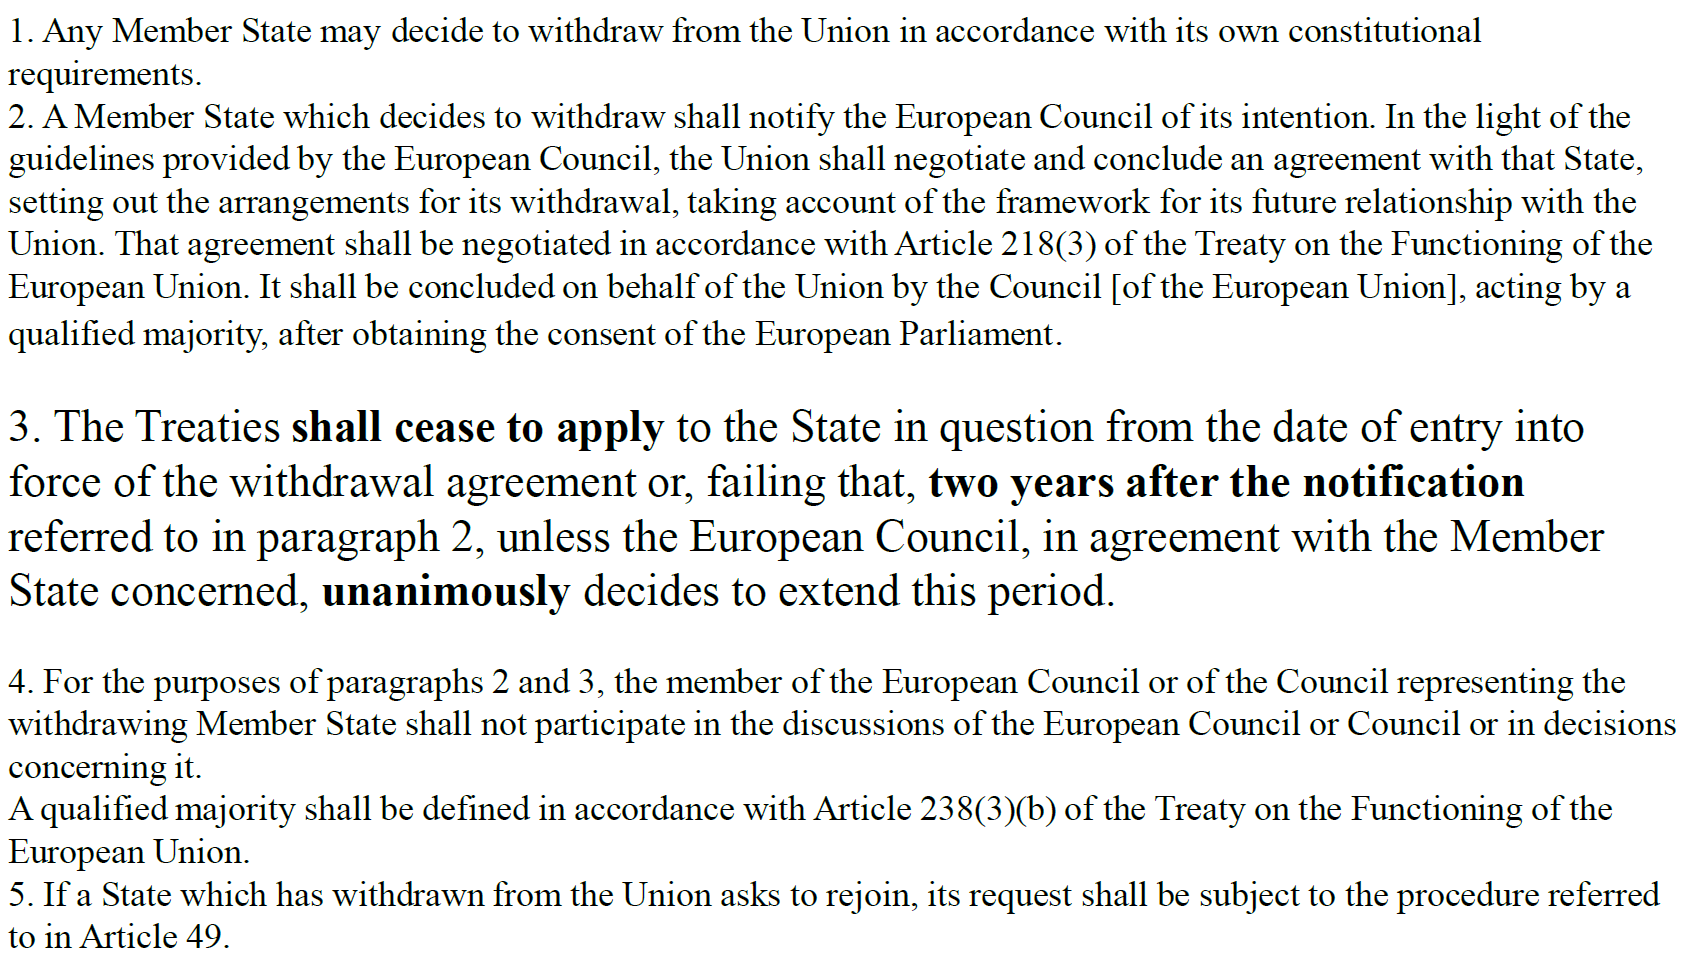
\includegraphics[width=0.85\textwidth]{Pictures/Art_50.png}
\end{figure}

\hrule

\paragraph{b) Negotiations}

\subparagraph{b1) Withdrawal Agreement}

What happened in the negotiations for the Withdrawal Agreement?

\begin{itemize}
    \item EU behaved professionally: EU defined and dominated Art 50.
        \begin{itemize}
            \item No negotiation without notification (according to art. 50)
            \item No future relationship without divorce agreement
            \item No divorve agreement without questions settled regarding:
                \begin{itemize}
                    \item Payments
                    \item Citizens' rights
                    \item Irish border
                \end{itemize}
        \end{itemize}
    \item UK had a bad start
        \begin{itemize}
            \item "We will negotiate the terms of the new deal before we start
                any legal process to leave" (according to Brexit campaign 2016)
            \item UK proposals violated the "no-cherry-picking"-prescription
                ("indivisibility of the 4 freedoms")
        \end{itemize}
    \item PM had a difficult job to come up with a clear UK position:
        \begin{itemize}
            \item Remainers wanted a second referentum
            \item Hardliner wanted a no-deal
            \item Soft-Brexit did not have a clear vision what was feasible and
                desirable
        \end{itemize}
    \item PM made two major mistakes:
        \begin{itemize}
            \item Substansive mistake: "Cherry-picking" and not well precooked
                with EU Council
            \item Tactical Mistake: Accepted of the 22.11.2018 draft agreement,
                containing the "backstop"
        \end{itemize}
    \item EU had a tough position:
        \begin{itemize}
            \item EU offended by the UK
            \item "Alcatraz-strategy"
            \item Veto-right for the EU regarding exit from EU Customs Union
            \item Professional way of negotiating:
            \item "An extension [of the deadline] will be something that
                extends uncertainty - and thus uncertainty has a cost"
        \end{itemize}
\end{itemize}

\subparagraph{b2)}

All in all there are 11 negotiation blocks (eg Transportation, Energy Goods,
Legal, etc). How did the negotiations for the Cooperation Agreement start?

\begin{itemize}
    \item Starting positions in a nutshell:
        \begin{itemize}
            \item UK:
                \begin{itemize}
                    \item Free trade agreement based on Canada-EU agreement
                    \item No involvement of EU institutions and no obligation
                        to take over new pieces of EU acquis
                    \item Goal to finish negotiations by end of the year
                \end{itemize}
            \item EU:
                \begin{itemize}
                    \item "Given the UK's geographic proximity and economic
                        interdependence with the EU27, the future relationship
                        will only deliver in a mutually satisfactory way if it
                        includes robust guarantees which ensure a level playing
                        field."
                    \item Same regulatory conditions and their continuity over
                        time: Uk should sign up to set of commitments "\dots
                        including all future EU rules on state aid and a 'status
                        quo' deal for access to UK fishing grounds, as the price
                        for agreeing a 'zero tariff, zero' quota trade deal."
                    \item Same monitoring rules: EU proposal very similar to the
                        one forwarded to Switzerland.
                \end{itemize}
        \end{itemize}
\end{itemize}

\paragraph{c) Results}

\subparagraph{c1) Withdrawal Agreement}

\begin{itemize}
    \item Key points:
        \begin{itemize}
            \item \underline{'Divorce bill'}: The agreement ensures that UK and EU honour
                all financial obligations undertaken while UK was an EU member
                $\rightarrow$ the financial settlement estimated at $\sim$
                GBP 30bn
            \item \underline{Protocol on Northern Ireland (NI)}: NI continues to align
                with EU rules on goods in order to avoid a hard border on the
                island, protecting the island economy and honoring the Good
                Friday Agreement $\rightarrow$ essentially NI remains at the
                same time a part of the EU's customs union (for regulatory
                purposes) and UK's customs territory (for UK's free trade
                agreements with third parties)
            \item \underline{Citizens' rights}: the life choices of over 3 million
                EU citizens in the UK and over 1 million UK nationals in
                EU countries have to be protected while safeguarding their
                right to stay $\rightarrow$ Independent Monitoring
                Authority (IMA).
            \item \underline{Transition period}: During the transition until 31 De 2020,
                the status quo will be maintained; the UK and EU may agree
                to a single extension of up to one or two years before 1 July
                2020. $\rightarrow$ Implications of Covid-19 crisis?
        \end{itemize}
\end{itemize}

\subparagraph{c2) Cooperation Agreement}

\begin{itemize}
    \item Key points:
        \begin{itemize}
            \item \underline{Trade}: Goods traded between EU and UK won't face new tariffs
                and quotas. However, new procedures introduced on borders such
                as safety checks and customs declarations (e.g. for rules of
                origin) $\rightarrow$ Doing business across UK and EU becomes
                more costly and burdensome.
            \item \underline{Services}: UK businesses offering services (banking,
                architecture, accounting) lose automatic access to EU markets and
                vice versa, no automatic recognition of professional qualifications
                (e.g. for doctors). $\rightarrow$ Rather then follwoing one set of
                rules for the whole EU, UK businesses need to comply with regulations
                in each individual country. EU and UK have pledged future dialogue
                on access in services sector, especially concerning financial services.
            \item \underline{Mobility}: UK nationals no longer have the freedom to work,
                study, start a business or live in the EU and vice versa. Visas required
                for stays longer than 90 days.
            \item \underline{Dispute settlement}: No role in the UK for the European
                Court of Justice (ECJ). Disputes that cannot be resolved between UK
                and EU are referred to an international tribunal instead.
                $\rightarrow$ Ending the role of ECJ was a key UK demand, for Brexit
                supporters it meant to "take back control" of its laws. ECJ retains
                some role in Northern Ireland, because it continues to follow some
                EU trade rules.
            \item \underline{Other points}: covering level playing field in environmental,
                social, and labour standards, education, fishing, security and data,
                education and other areas.
        \end{itemize}
\end{itemize}

\paragraph{d) Comments}

Eight Lessons from Brexit, from a Swiss point of view.

\begin{enumerate}[1)]
    \item Influence of UK-EU negotiations on bilateral efforts between Switzerland
        and EU obvious.
    \item Deadlines usually put pressure on smaller negotiating partners:
        \begin{itemize}
            \item The deadline of 29 March probably led May to accept an immature
                or unbalanced treaty text in November 2018.
            \item Evidence: lack of support in parliament.
        \end{itemize}
    \item "Best alternative to negotiated agreement" proofs to be tactically wise:
        \begin{itemize}
            \item little advantage for May by taking no deal solution off the
                table, because this gave the EU stong leverage
            \item Johnson brought (i) BATNA back into play and (ii) made new
                proposals; EU was suddenly ready to resume negotiations
        \end{itemize}
    \item Elaborating concrete options brings weaker negotiating partners further
        instead of just saying no:
        \begin{itemize}
            \item Last Brexit negotiation rounds show as soon as Johnson presented
                a new idea (simultaneous integration of Northern Ireland into the
                EU international market and the UK customs union) did the possibility
                of concluding the agreement arise
        \end{itemize}
    \item Proposals only have a chance if they do not harm the vital interests
        of the negotiating partners:
        \begin{itemize}
            \item EU right of veto on Irish border issue;
            Only the correction of the backstop solution and the protection
            of Irish interests made a majority in the British Parliament possible
            in the first place
        \end{itemize}
    \item The Cooperation Agreement clears the path for future agreements.
        \begin{itemize}
            \item In this sense the EU-UK partnership could be similar to the
                EU-Swiss bilateral way.
        \end{itemize}
    \item The Cooperation Agreement brings a new balance between sovereignty and
        cooperation.
        \begin{itemize}
            \item Compared to the status quo antea a bit more sovereignty and
                less market access. Whether this new balance is better than the
                old one can be only judged in a later phase and of course is
                primarily up to the UK to evaluate this question.
        \end{itemize}
    \item Brexit could have far reaching consequences on the unity of the UK.
        \begin{itemize}
            \item Scotland independence referendum; Status of Northern Ireland
        \end{itemize}
\end{enumerate}


\subsection{Nuclear Waste - Framework for Remuneration Negotiations}

In the beginning of 2017, we had been mandated by the Swiss Federal Office
for Energy to develop a framework for the negotiation of remuneration
payments to the siting region of a deep geopolitical repository for the
disposal of nuclear waste.

\paragraph{a) Background}

\begin{itemize}
    \item Radioactive waste is produced in
        \begin{itemize}
            \item Nuclear power plants (32.8\% of Swiss electricity production)
            \item Industry
            \item Medicine
            \item Science
        \end{itemize}
    \item 26\% comes from Industry, Medicine, Science and 74\% come from
        Nuclear Power Plants
    \item Estimated to amount finally to approximately 87'000 m$^3$
    \item $8\%$ High-level waste (HLW), $2\%$ Alpha-toxic waste (ATW),
        $90\%$ Low- and intermediate-level waste (L/ILW)
    \item The law defines that:
        \begin{itemize}
            \item Radioactive waste, produved in Switherland, has to be
                disposed of in Switzerland.
            \item The waste producers have to pay for the disposal.
            \item Radioactive waste has to be disposed of in such a way that
                the long-term protection of people and the environment is
                ensured
            \item Radioactive waste has to be disposed of ina deep geological
                repository.
        \end{itemize}
\end{itemize}

The search for a siting region is a long process.

\begin{itemize}
    \item 1972, the National Cooperative for the Disposal of Radioactive
        Waste (Nagra) was founded
    \item 1994 Wellenberg was chosen for a L/ILW repository
    \item 1995 Nidwalden voters rejected the concession with $51.9\%$
    \item 2002 Nidwalden voters rejected the exploratory tunnel with $57.7\%$
    \item 2003 New Nuclear Energy Act (Kernenergiegesetz)
    \item 2008 Sectoral Plan Deep Geological Repositories
\end{itemize}

\paragraph{b) Negotiation}

\begin{itemize}
    \item Developing a negotiation framework
    \item Negotiation are voluntarily, therefore the framework has only
        a value if all parties accept it. These are:
        \begin{itemize}
            \item Waste Producers
            \item Siting Regions
            \item Cantons
        \end{itemize}
    \item The development of the negotiating framework itself is a negotiation
    \item Our task: not so much to just make the best proposals, but rather
        to draw up the rules of the game to which all parties would agree in
        the end.
\end{itemize}

Difficulties:
\begin{itemize}
    \item Concerning the form:
        \begin{itemize}
            \item Framework had to be established in consensus with all
                involved parties.
        \end{itemize}
    \item Concerning the substance:
        \begin{enumerate}[i.]
            \item in the beginning, negotiation objective was not clear
                \begin{itemize}
                    \item It was not clear if one would negotiate about
                        compensation payments and about remuneration payments
                        (definition in the documents leaves some ambiguity)
                    \item Art. 1 Negotiation Objective:
                        Objective of the negotiation is the regulation regarding
                        remuneration payments and if appropriate about possible
                        compensations.
                \end{itemize}
            \item in the beginning, negotiation parties were not clear
                \begin{itemize}
                    \item Waste producer (role of federal state)
                        \begin{itemize}
                            \item The power plant operators insisted on the
                                participation of the federal state (responsible
                                for insustry, medicine, and science).
                                \begin{itemize}
                                    \item Everything happens unter the assumption that
                                        all waste producers (including the federal state)
                                        will participate in the payment.
                                    \item In what form the federal state will participate
                                        in the payment is still unknown. Als unknown is, if
                                        the federal state will participate in the negotiations.
                                        (no contract at the expense of a third party)
                                \end{itemize}
                        \end{itemize}
                    \item Competences of siting regions
                        \begin{itemize}
                            \item A region is not a legal entity in Switherland
                                $\rightarrow$ The municipalities will have to sign
                                the contract and will have to negotiate.
                        \end{itemize}
                    \item Participation of Germany
                        \begin{itemize}
                            \item Germany wanted to be a part of the negotiations
                                $\rightarrow$ There is one additional seat in the
                                delegation of the municipalities reserved for Germany.
                        \end{itemize}
                \end{itemize}
            \item Beginning of the negotiatio was not clear
                \begin{itemize}
                    \item The waste producers wanted to start the negotiations late
                        and the regions wanted to start early.
                    \item The intention was that the negotiation parties are known
                        (region is selected), while at the same time giving the regions
                        enough time for their internal processes.
                    \item $\rightarrow$ Definition of an interval: The negotiations start
                        the earliest after [\dots] but not later than [\dots]. The two
                        reference points are not fixed dates but defined through the
                        process.
                \end{itemize}
            \item Entry into force of contract
                \begin{itemize}
                    \item One single municipality could block an agreement for the
                        whole region. $\rightarrow$ Therefore the contract comes
                        into force if
                        \begin{itemize}
                            \item all waste producers,
                            \item all cantons,
                            \item $60\%$ of all municipalities of a region and
                            \item $60\%$ of all infrastructure municipalities
                        \end{itemize}
                        agree within a period of two years.
                \end{itemize}
            \item Commitment of the negotiation framework
                \begin{itemize}
                    \item The framework could not be legally binding binding
                        but should still have a clear commitment.
                    \item \underline{Decleration}: The signatories [\dots]
                        confirm their firm intention to recommend to the
                        responsible authorities of their institutions to use
                        this negotiation framework as a basis for the negotiations
                        of remunerations / compensations.
                \end{itemize}
        \end{enumerate}
\end{itemize}


\paragraph{c) Results}

\begin{itemize}
    \item Declaration (2 sentences)
    \item 20 signatuers
    \item Negotiation framework (6 pages including front page and preable)
    \item 12 articles:
        \begin{itemize}
            \item Negotiation objective
            \item Negotiation subject
            \item Usage
            \item Negotiation parties
            \item Begin of negotiation
            \item Frequency of meetings
            \item Chair, negotiation secretariat, and editing of contract
            \item Arrangement of meetings
            \item Communication
            \item Conclusion of negotiation
            \item Entry into force of contract
            \item Other closing provisions
        \end{itemize}
\end{itemize}

\paragraph{d) Comment}

You work with people:
\begin{itemize}
    \item Building a good and respectful working relationship makes the process easier.
    \item In our situation it was furthermore very important to treat every perty equal
        (same rights, communication, and information)
    \item Always listen very carefully and try to understand the sensitives of the parties.
    \item A negotiator is always under pressure from his constituency at home.
    \item You should negotiate with the people who can make the decisions.
    \item It was always essential for us to have a close contact with all involved parties
        (sometimes this means talking beck and forth five times a day, sometimes it means
        to have a emergenfy meeting at 7 a.m. in another city).
\end{itemize}
Be always well prepared
\begin{itemize}
    \item Know the subject well.
    \item Be prepared for different developments in a negotiation and have
        varying proposals ready.
    \item If the process is stuck, generate new alternatives which try to
        circumvent the obstacle.
    \item Be skeptical and also plan for the worst case.
\end{itemize}
Keep calm
\begin{itemize}
    \item There is often an escalation in the end of negotiatio. Keep calm
        and try to solve emerging problems.
    \item Know when to be firm in tone.
\end{itemize}
Have a good working procedure
\begin{itemize}
    \item After an initial round, try to work with a negotiation text.
    \item Conflicting views or parts which are still to debate can be notated
        in square brackets. They are then later resolved.
    \item Don't vote on specific points or formulation. Work on a consensus basis.
    \item Nothing is agreed until everything is agreed.
\end{itemize}

\subsection{US-Swiss UBS Deal}

\paragraph{a) Background}

\begin{itemize}
    \item 18. Feb. 2009: UBS $\leftrightarrow$ Dep. of Justive (DoJ),
        Deferred Prosecution Agreement
        \begin{itemize}
            \item Penalty of \$ 780'000'000
            \item Obligation to hand out 52'000 names of US-clients
        \end{itemize}
    \item Problem: Conflict of jurisdictions. Choice of UBS would be:
        \begin{itemize}
            \item Either to violate US Law (by not handing out the names)
            \item Or to violate Swiss Law (by handing out the names)
        \end{itemize}
\end{itemize}

\paragraph{b) Negotiation}

\begin{itemize}
    \item 22. June 2009: First meedint in Washington DC
    \item Several rounds of negotiations
    \item 31. July 2009: Agreement in principle on ministerial level
    \item 19. August 2009: Signing and entry into force
\end{itemize}

Three key problems in the negotiation:
\begin{enumerate}[1)]
    \item To convince the US-side to negotiate in the first place
        \begin{itemize}
            \item We had to convince the IRS that in case they would force UBS
                to hand out 52'000 names, Swiss police authority would confiscate
                UBS data ("Blocking Order" by the Swiss government)
            \item We explained in detail that the government ordinance (Blocking Order)
                could be put into force within one or two hours
            \item This would have lead to a classical lose - lose situation (even though
                the "lose part" of Switherland would have been bigger than the one of
                the US)
            \item As a consequence, the US preferred the win - win: $\rightarrow$ start negotiation
        \end{itemize}
    \item How to give clients' names on based existing law?
        \begin{itemize}
            \item We can only give the names according to swiss law.
        \end{itemize}
        \begin{figure}[H]
            \centering
            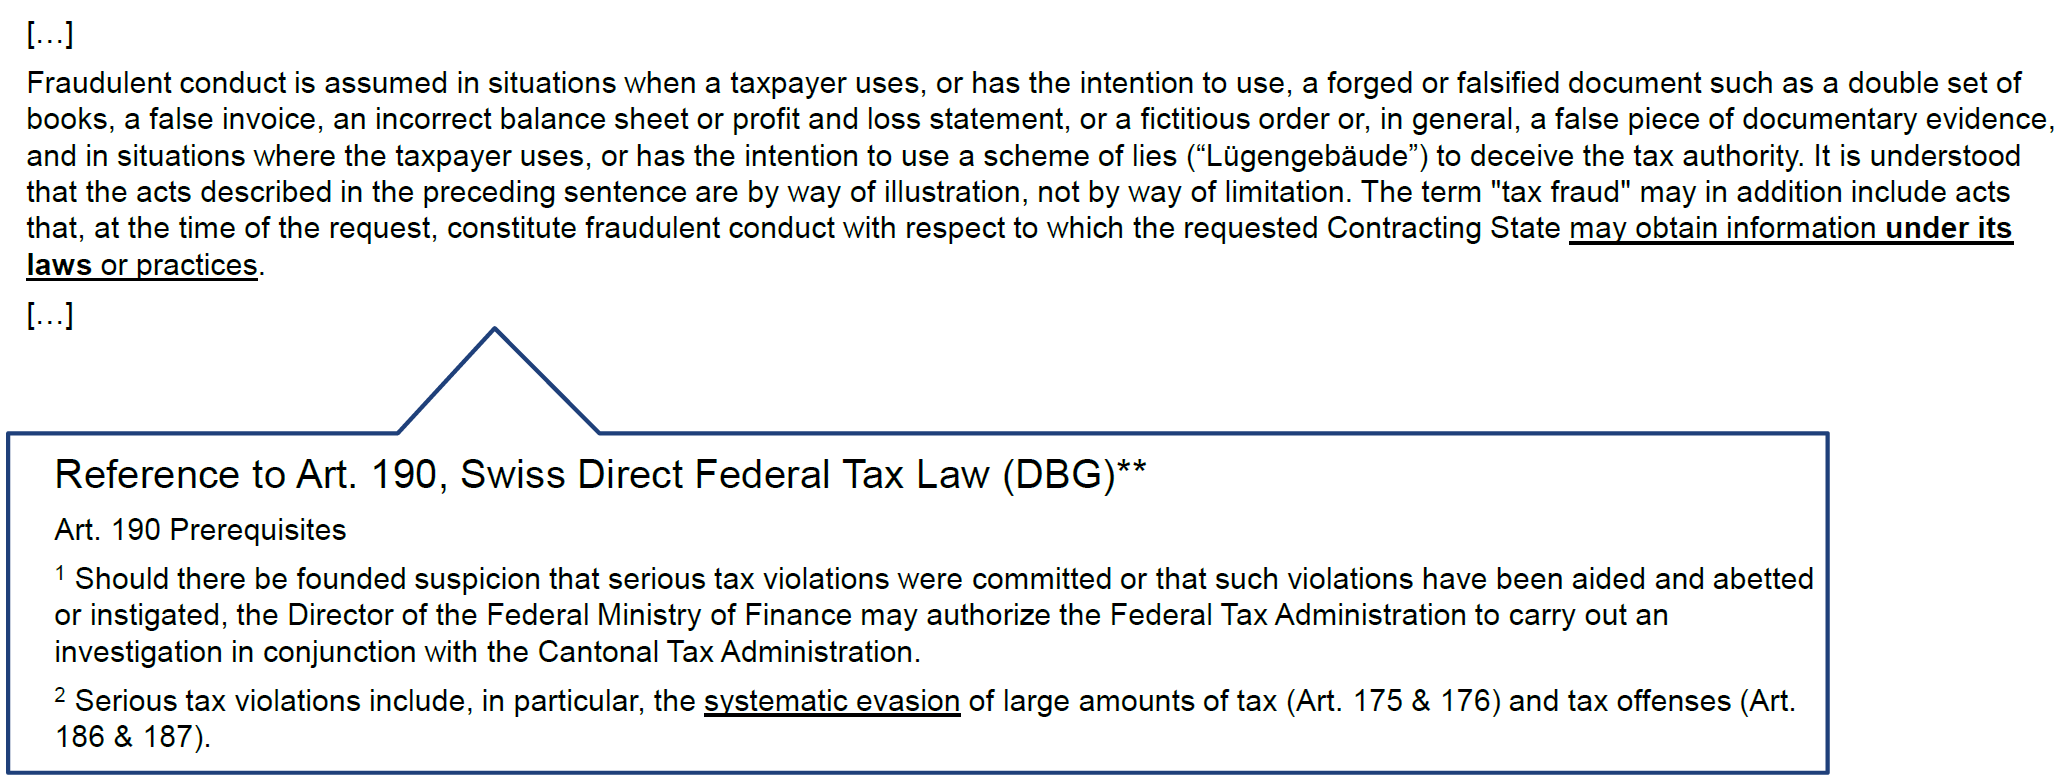
\includegraphics[width=\textwidth]{Pictures/UBS_USA_problem_2.png}
        \end{figure}
        Underlined phrase: National treatment. We offer to the other government
        to deal with their request as if they would be a national authority.
        We treat them in the same way as we treat out own citizens.
    \item Independence of the Swiss courts: What shall be done if due to
        appeals the expected number of names (bank accounts) cannot be reached?
        (The expected number was estimated 4450)
        \begin{itemize}
            \item Rebalancing measures - inspired by the EEA-concept
            \item Article 114 EEA (European Economic Area)
                \begin{enumerate}[1.]
                    \item If a safeguard measure taken by a Contracting Party creats
                        an imbalance between the rights and obligations under this
                        Agreement, any other Contracting Party may towards that
                        Contracting Party take such proportionate rebalancing
                        measures as are strictly necessary to remedy to imbalance.
                        Priority shall be given to such measures as will least
                        disturb the functioning of the EEA.
                    \item The Procedure under Article 113 shall apply.
                \end{enumerate}
            \item If the expected number could not be reached, the DoJ would be
                allowed to take rebalancing measures. In the sense, to go back
                to the terms of the DPA.
        \end{itemize}
\end{enumerate}

\paragraph{c) Result}

\begin{itemize}
    \item Agreement between Switzerland and USA on the request for information
        from the Internal Revenue Services of the USA regarding UBS, a corporation
        established under the laws of the Swiss Confederation
        \begin{itemize}
            \item Initialed: 12. August 2009
            \item Signed: 19. August 2009
        \end{itemize}
    \item Swiss Laws respected
    \item US got names on the basis of the treaty requests
    \item Integration of a European concept of Rebalancing into an American
        treaty. Special for the US.
\end{itemize}

\paragraph{d) Comment}

\begin{itemize}
    \item Creative interpretation of texts
    \item Negotiate, not just "yes" of "no"
\end{itemize}

\subsection{Overview}

\begin{figure}[h]
    \centering
    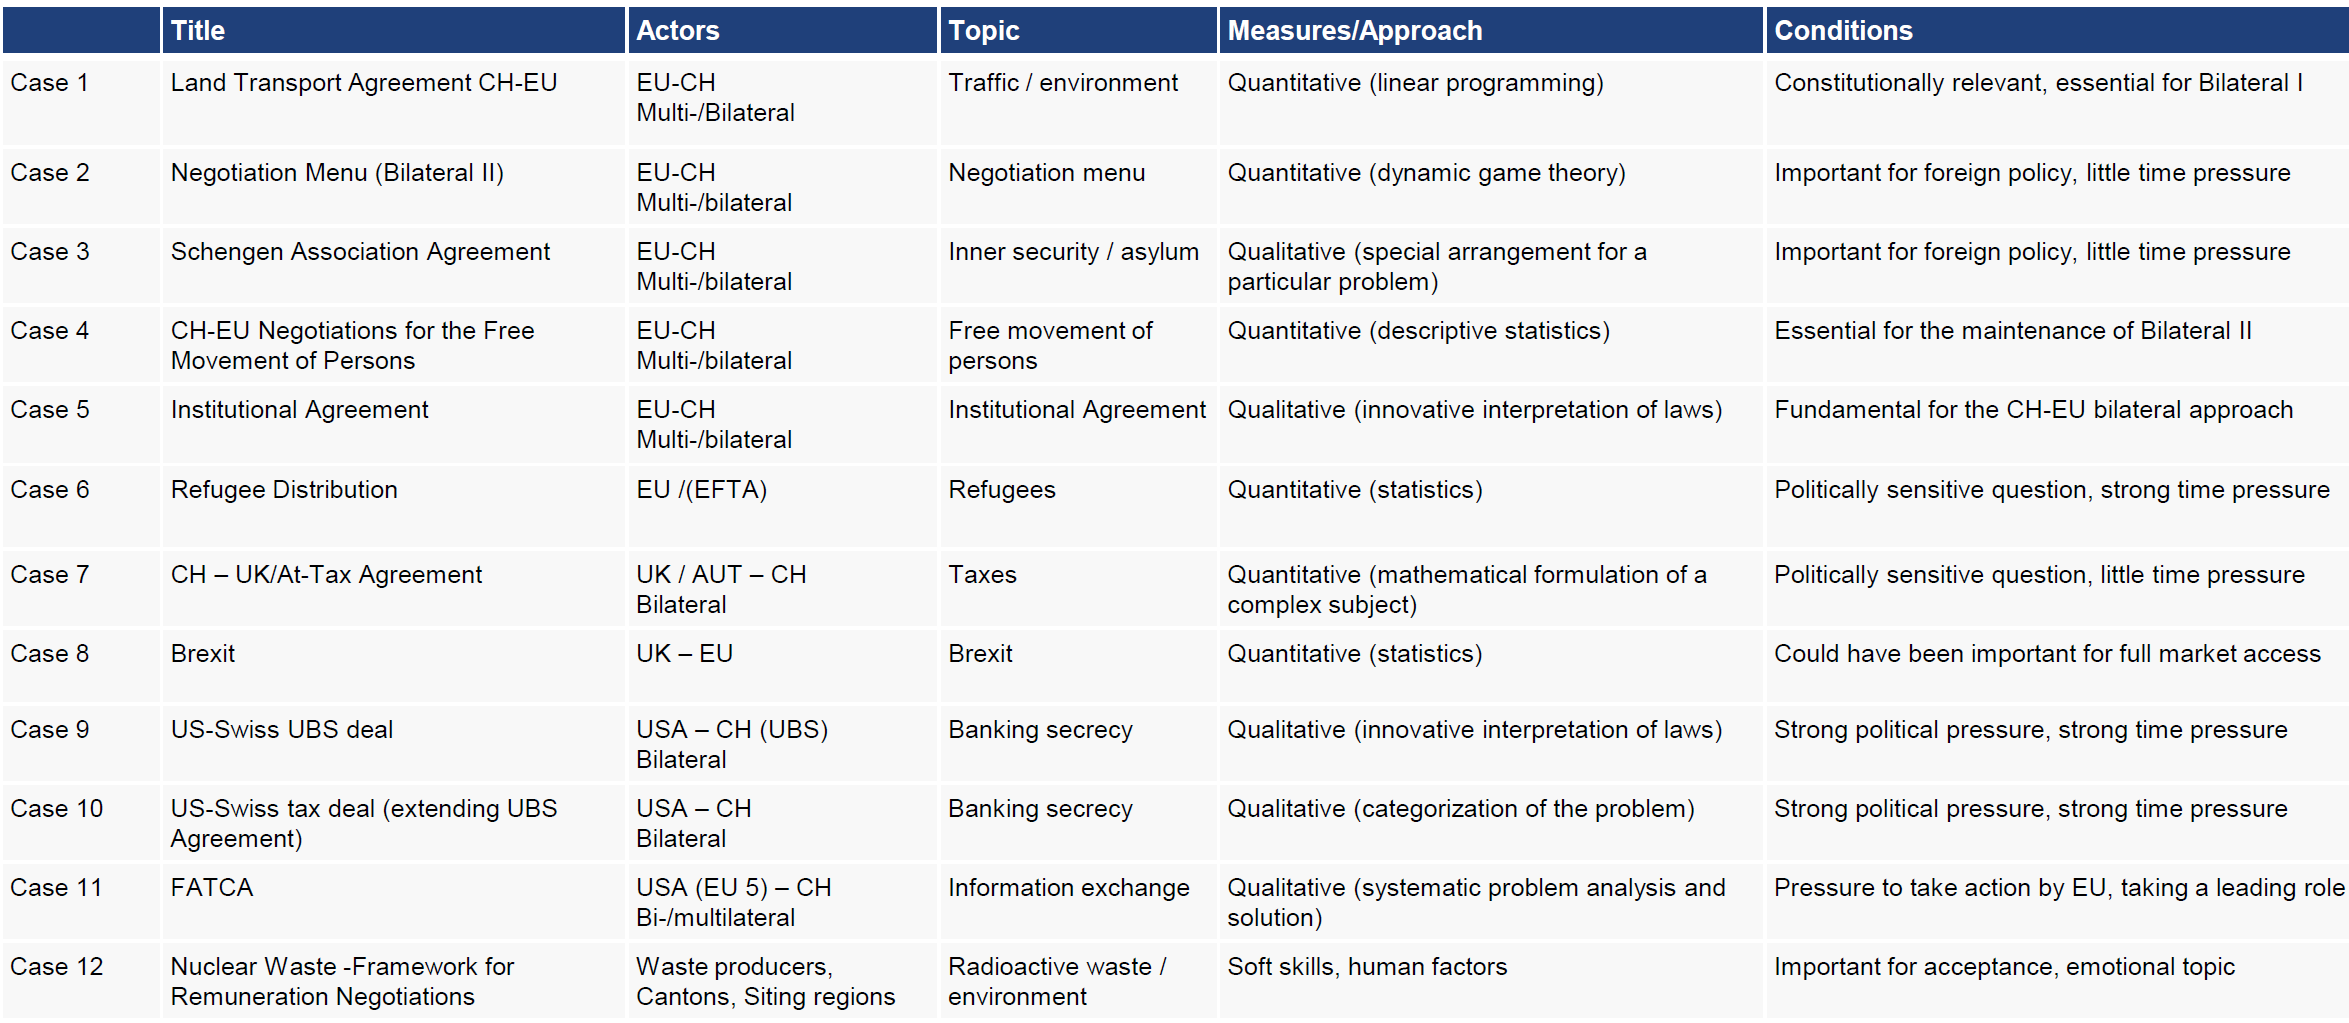
\includegraphics[width=1.05\textwidth]{Pictures/Overview_Case_studies.png}
\end{figure}

\pagebreak

In all Cases (1-12) there is:
\begin{itemize}
    \item a difficult intergovernmental negotiation problem (exept case 12)
    \item a reduction of the problem to its formal structure
    \item application of heuristic methods
    \item application of systematic/methodological thinking
    \item the use of mathematical methods (Where appropriate/possible (cases:
        Land Transport,Bilateral \uproman{2}, Free Movement of Persons, Refugee
        Distribution, CH-UK Tax agreement, Brexit))
\end{itemize}
